\documentclass[bibliography=totoc, listof=totocnumbered]{scrartcl}
    % General document formatting
    %\usepackage[margin=0.7in]{geometry}
    %\usepackage[parfill]{parskip}
    \usepackage[utf8]{inputenc}
    %\usepackage[headsepline,footsepline]{scrpage2}
    \usepackage[onehalfspacing]{setspace}
    \usepackage{times}
    \usepackage{graphicx}
    \usepackage{fancyhdr}
    \usepackage{lastpage}
    \usepackage[affil-it]{authblk}
    \usepackage[australian,british]{babel}
    \usepackage[ddmmyyyy]{datetime}
    \usepackage[toc,page]{appendix}
    \graphicspath{ {images/} }
    \usepackage[style=numeric,sorting=none,backend=bibtex]{biblatex}
    \addbibresource{citations.bib}
    \usepackage[citecolor=black]{hyperref}

% Header and Footer Formatting-----------------------------------------------------------------------
%   Formatting of Header and Footer
% ---------------------------------------------------------------------------------------------------
%\pagestyle{scrheadings}
%\clearscrheadfoot
%\ohead{\headmark}
%\ofoot{\pagemark}

% TODO: make itemize neater

% Center all images
\makeatletter
\g@addto@macro\@floatboxreset\centering
\makeatother

\pagestyle{fancy}
\renewcommand{\dateseparator}{.}

\lhead{Technical Article}
\rhead{PSIT4}

\fancyfoot[L]{\footnotesize \today }
\fancyfoot[C]{\footnotesize Page \thepage\ of \pageref{LastPage}}


% Title Page Information-----------------------------------------------------------------------------
%   These are the informations printed on the title page of the article
% ---------------------------------------------------------------------------------------------------
\fancypagestyle{firstpage}
{
	\renewcommand{\headrulewidth}{0pt}
	\fancyhf{}
}\fancyfoot[R]{\footnotesize IT15ta\_ZH Group trckr}

\begin{document}
\begin{titlepage}
\thispagestyle{firstpage}
\centering

\includegraphics[width=0.3\textwidth]{logo}\par
\vspace{1cm}

{\scshape\LARGE Project trckr \par}
\vspace{0.3cm}

{\scshape IT15ta\_ZH - PSIT4\par}
\vspace{0.5cm}
Ankeshian, Gabriel\\
\texttt{ankesgab@students.zhaw.ch}

\vspace{0.2cm}
Balidis, Dimitri\\
\texttt{baliddim@students.zhaw.ch}

\vspace{0.2cm}
Christen, Luca\\
\texttt{chrisluc@students.zhaw.ch}

\vspace{0.2cm}
Jossi, Savino\\
\texttt{jossisav@students.zhaw.ch}

\vspace{0.2cm}
Milenkovic, Daniel\\
\texttt{milendan@students.zhaw.ch}

\vspace{0.2cm}
Nominato, Angelica Helena Moreira Alves\\
\texttt{moreiane@students.zhaw.ch}

\vspace{0.2cm}
Pacassi Torrico, David\\
\texttt{pacasdav@students.zhaw.ch}

\vfill

% Bottom of the page
	{\large \today\par}
\end{titlepage}

% Proofreading Checklist
% * avoid passive voice
% * succinct sentences
% * use active voice
% * did I say don't use passive voice?

% Abstract----------------------------------------------------------------------
%   This is the abstract of the technical article
% ------------------------------------------------------------------------------
\begin{abstract}
  The main goal of the present article is to describe the idea, goals and main
  functionalities of the web-based application trckr. We developed trckr for
  % Since we want trckr to be all lowercase, we avoid using it at the start of
  % the sentence
  everyone who works on a project and needs an intuitive and simple web tool to
  accurately track their time spent on different tasks.
  % Hint: Empty line makes a paragraph which is semantically different from the
  % forced \\ newline (and much neater)

  The back-end is written in Python with the help of the web application
  framework Django and the front-end with the Javascript UI framework Vue.js.
  Both technologies were new to most team members, but all members have proven
  themselves motivated to learn these skills which was ultimately a benefit to
  the outcome of the project.

  In order to compete with similar tools and web services, trckr focuses on
  performance and usability. To distinguish trckr from the competition, many
  features are planned to manage projects and tasks in a user-friendly manner.
  This will allow the user to leverage trckr to handle the ever-increasing
  complexity in project management and task tracking found in large companies.
  Despite targeting large companies, trckr will remain open-source and anyone
  can contribute to the codebase who might wish to do so.
\end{abstract}

\clearpage

\section{Introduction}
Time and task tracking are important activities in many businesses to gain
insights on the productivity of a team. Appropriate tools allow easier and more
accurate time tracking. Many processes and methods have been developed in the
past to cover this need. Unfortunately most of them only address a certain need
or have been fine-tuned to fit a specific company or team. This not only leads
to a loss of experience that could have been leveraged by other teams but is
also not generic enough to adapt to different processes, causing other companies
to inappropriately adapt to the tool instead of the tool adapting to the
company.

\subsection{Objectives}
The goal with trckr is to develop and distribute a time tracking web application
that is easy to both understand and use. The most important non-functional
requirement is to focus on a small amount of steps for users to track all the
required information. This will keep the user engaged and increase the accuracy
of the provided data.

\subsection{Main Features}
The user is able to:
\begin{itemize}
    \item register and login to trckr
    \item create and edit projects
    \item create, track and edit tasks
    \item visit trckr on any device
\end{itemize}

\section{Architecture}
The trckr project consists of two separate applications. The business and data
layers are handled by the back-end application while the presentation layer is
implemented through the front-end application. The back-end provides a RESTful
API which is used by the front-end application to read and write the necessary
data.

This separation of concerns, achieved through the clear decoupling between the
front-end and back-end, allows for easy extensibility and fast development
cycles. Additionally, a single back-end is able to serve multiple client
applications without any further work required.

\begin{figure}[h]
    \includegraphics[width=8cm]{architecture}
    \caption{Architecture of trckr}
    \label{fig:architecture}
\end{figure}

\section{Technologies}
\subsection{Django}
Django is an open-source web framework written in Python.\cite{django} It
encourages fast, clean and simple development of web applications. One of the
main advantages is its fast setup, enabling the developer to create applications
swiftly through its Model-View-Presenter scheme. Django also comes with support
for various databases and follows the DRY (Don't Repeat Yourself) principle.

\subsection{PostgreSQL}
PostgreSQL is an open-source object-relational database.\cite{postgre} The
database is used to store all the data for trckr. PostgreSQL is fully supported
by Django and requires minimal configuration. The communication between the web
application and the database is done through Django's model layer.

\subsection{Docker}
Docker is a containerization platform that adds an abstraction layer between the
application environement and the underlying server infrastruture.\cite{docker}
This means that the whole back-end environment can be setup inside multiple
docker containers that can be run locally as well as on the server.

\subsection{Node.js}
Node.js is a Javascript runtime which brings Javascript to the server
environment.\cite{nodejs} It uses an event-driven and non-blocking I/O model for
maximum efficiency while still remaining lightweight. This makes node.js the
ideal technology to implement the server side of the trckr front-end application.

\subsection{Vue.js}
Vue.js is a progressive framework for building user interfaces.\cite{vuejs}
Vue.js is used mainly for its simplicity and the rather shallow learning curve
it provides unexperienced developers. The features of Vue.js allow
the creation of data structures that can easily be displayed on a website. This
and the ability to easily make calls to the back-end make it a good fit for
trckr.

\section{Results}

\subsection{API}
The back-end of the trckr application implements a RESTful API using the Django
REST framework. The API provides basic CRUD operations for all the entities
available in the database. There are five main endpoints to retrieve and save
data on the server: authentication, user, projects, tasks and time entries.
Except for the authentication and user endpoints, all endpoints need an
authentication token to be accessed.

\subsubsection{Endpoints}
\begin{description}
\item[authentication] allows users to retrieve an authentication token from the
  server to access the other parts of the API. Via this endpoint, one can also
  invalidate the token.
\item[user] is only used to create new user accounts.
\item[projects] allows users to create, read, update and delete projects and
  display all the tasks associated with a project.
\item[task] is used to create, read and update tasks for a given project. There
  is also a way to list all relevant time entries for a task.
\item[time entries] are also used to create, read, update and delete operations
\end{description}

Each object of an entity has a unique ID. This ID can be used to retrieve
information for that specific object by providing it in the URL when calling the
server. This is necessary when updating an object via a POST request.

\subsection{User Interface}
% SJ: I removed details about the implementation (receive a token) and rewrote
% to reflect the UX

When a user first opens up the trckr web application, the user is presented with
the login screen as shown in Figure \ref{fig:trckr-login}. For users who have
not yet registered an account, they can create one by clicking on "Register" and
entering their basic information, i.e. their username, password, email address
as well as first and last name (see Figure \ref{fig:trckr-register}).

\begin{figure}[h]
    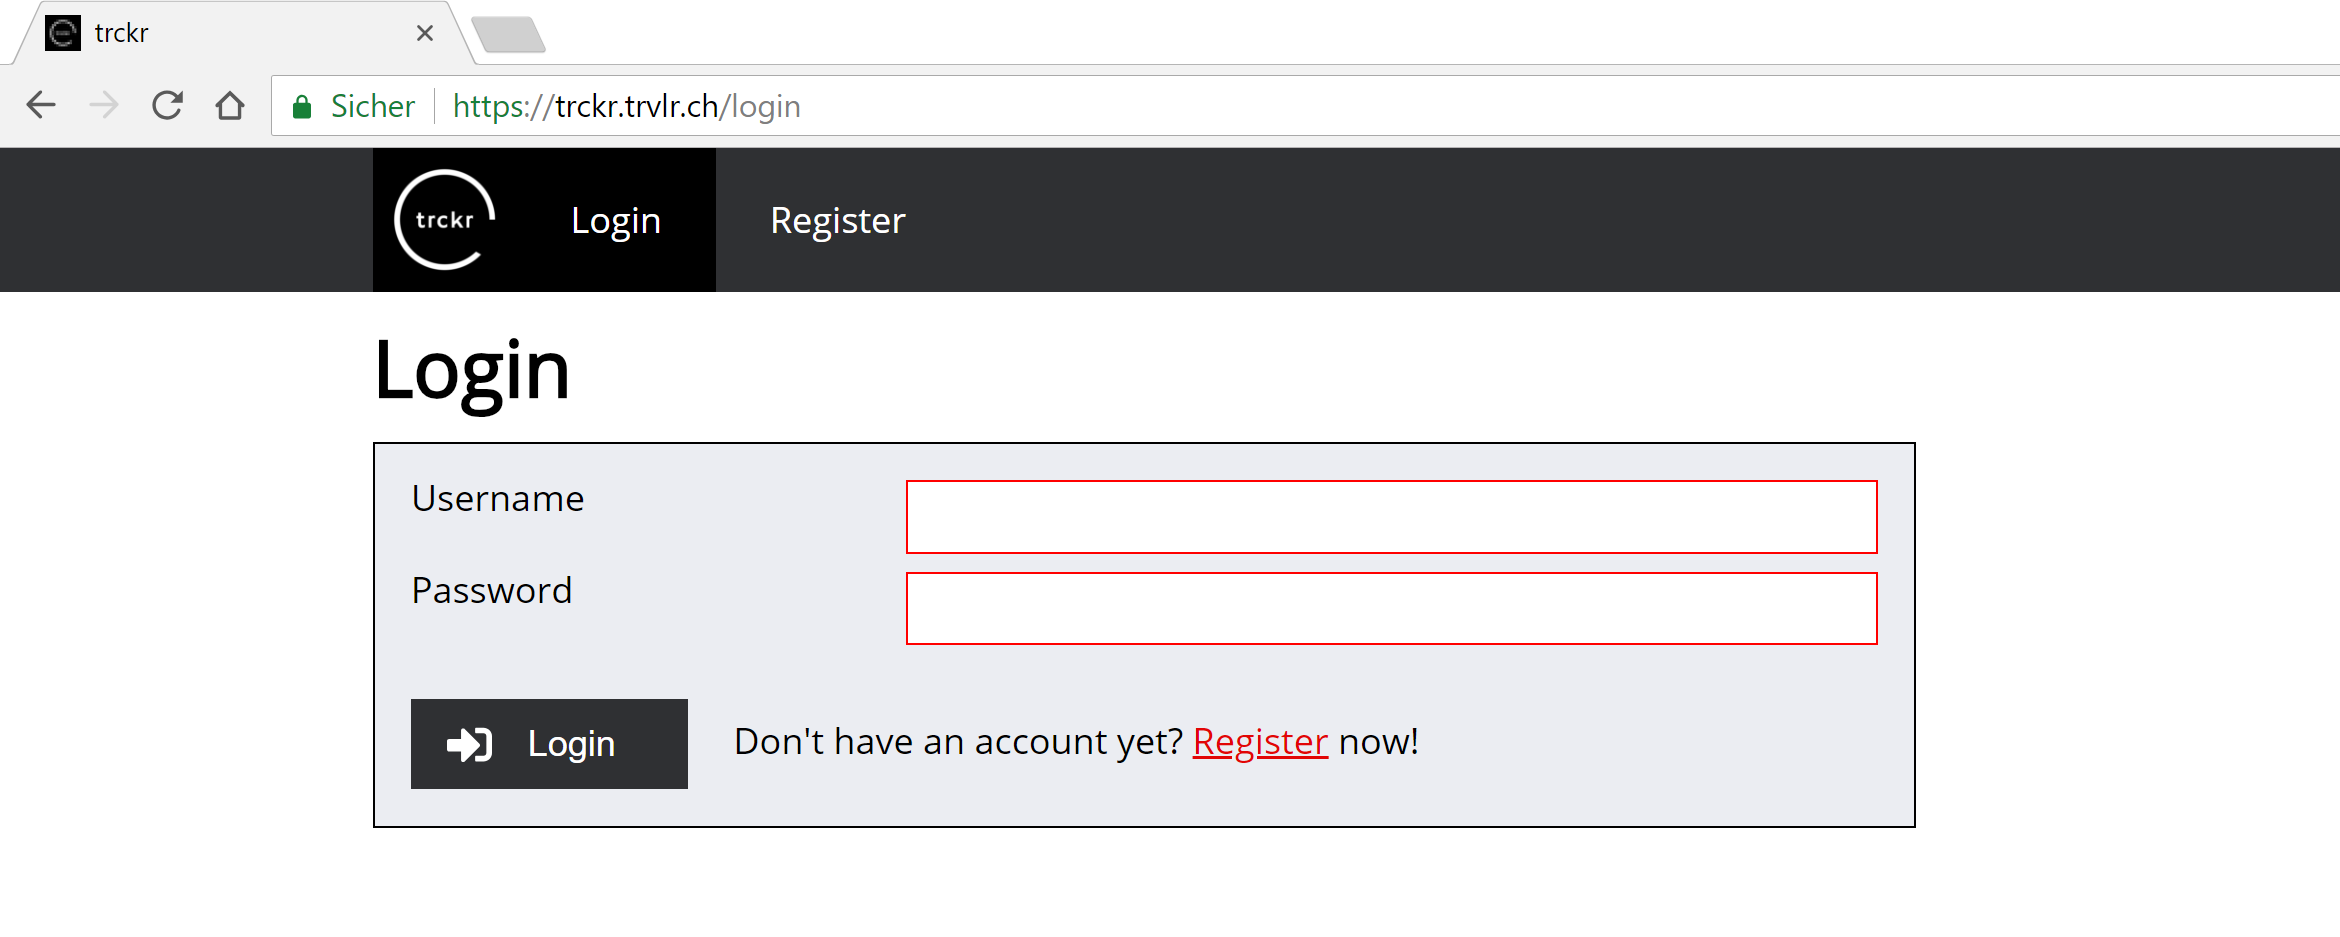
\includegraphics[width=0.8\textwidth]{trckr-login}
    \caption{The trckr login page}
    \label{fig:trckr-login}
\end{figure}

\begin{figure}[h]
    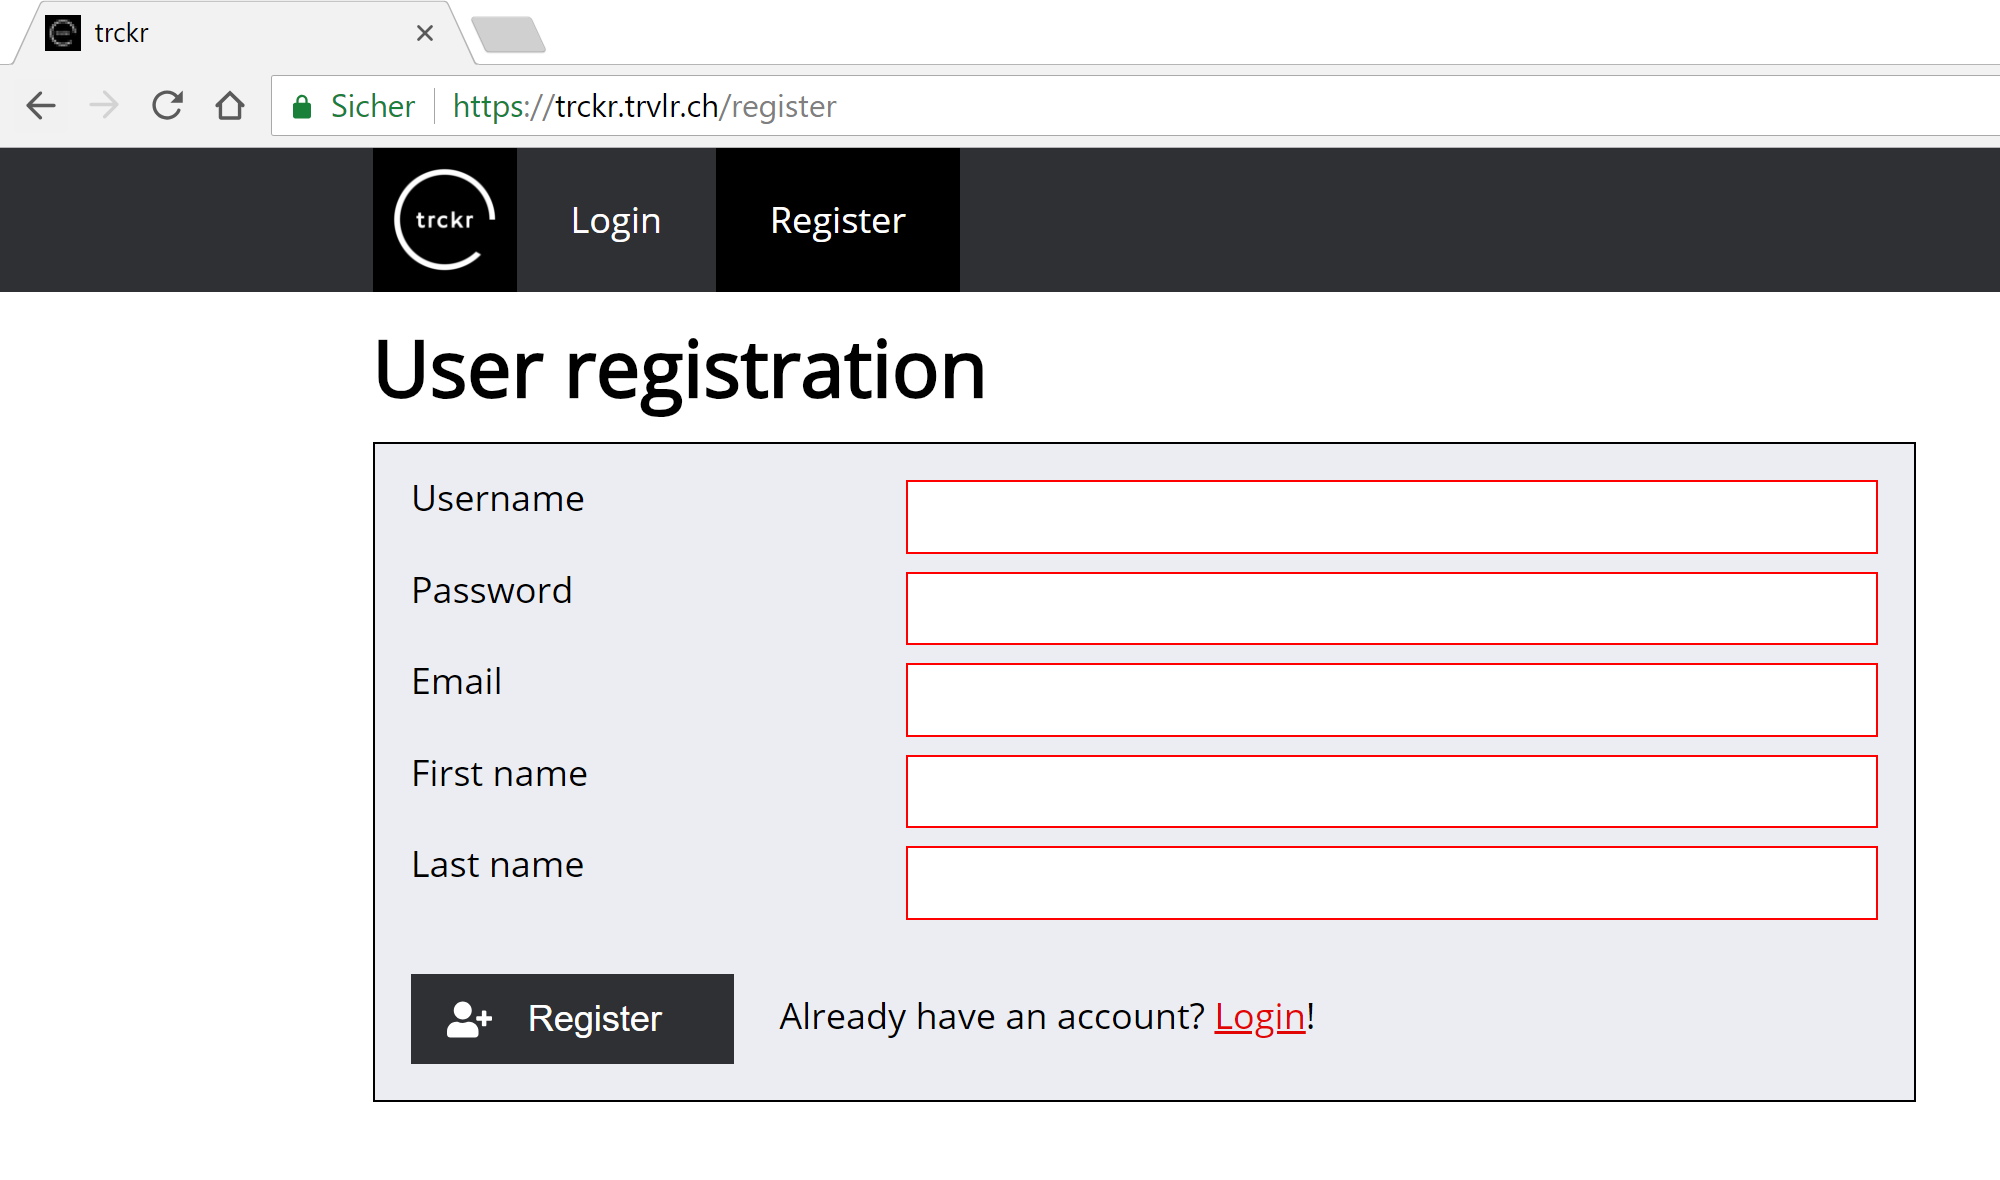
\includegraphics[width=0.8\textwidth]{trckr-register}
    \caption{The trckr registration page}
    \label{fig:trckr-register}
\end{figure}

Once the registration process has been completed, the user can log in at the
login page. After a successful login, the navigation bar at the top of the
interface will contain links to the dashboard, the projects page and the time
entries page as well as a logout button. The dashboard displays different graphs
to provide the user with a visual overview of their recent activities. This way
the user can easily see how much time was already tracked for each task and it
enables the user to quickly proceed with their work, whithout having to search
for a relevant task.
% TODO include figure once the dashboard is finished...

The projects page shows a table of all projects that the currently logged in
user is a part of; this can be seen in Figure \ref{fig:trckr-projects-table}.
There is a search box above the projects table that allows a user to filter for
a project or a group of projects containing the given keywords. To create a new
project, the user will have to navigate to the projects page and click the
"Create project" link which will open the project creation form. The user
specifies the name for the project and also has the option to enter a
discription (see Figure \ref{fig:trckr-create-project}).

\begin{figure}[h]
    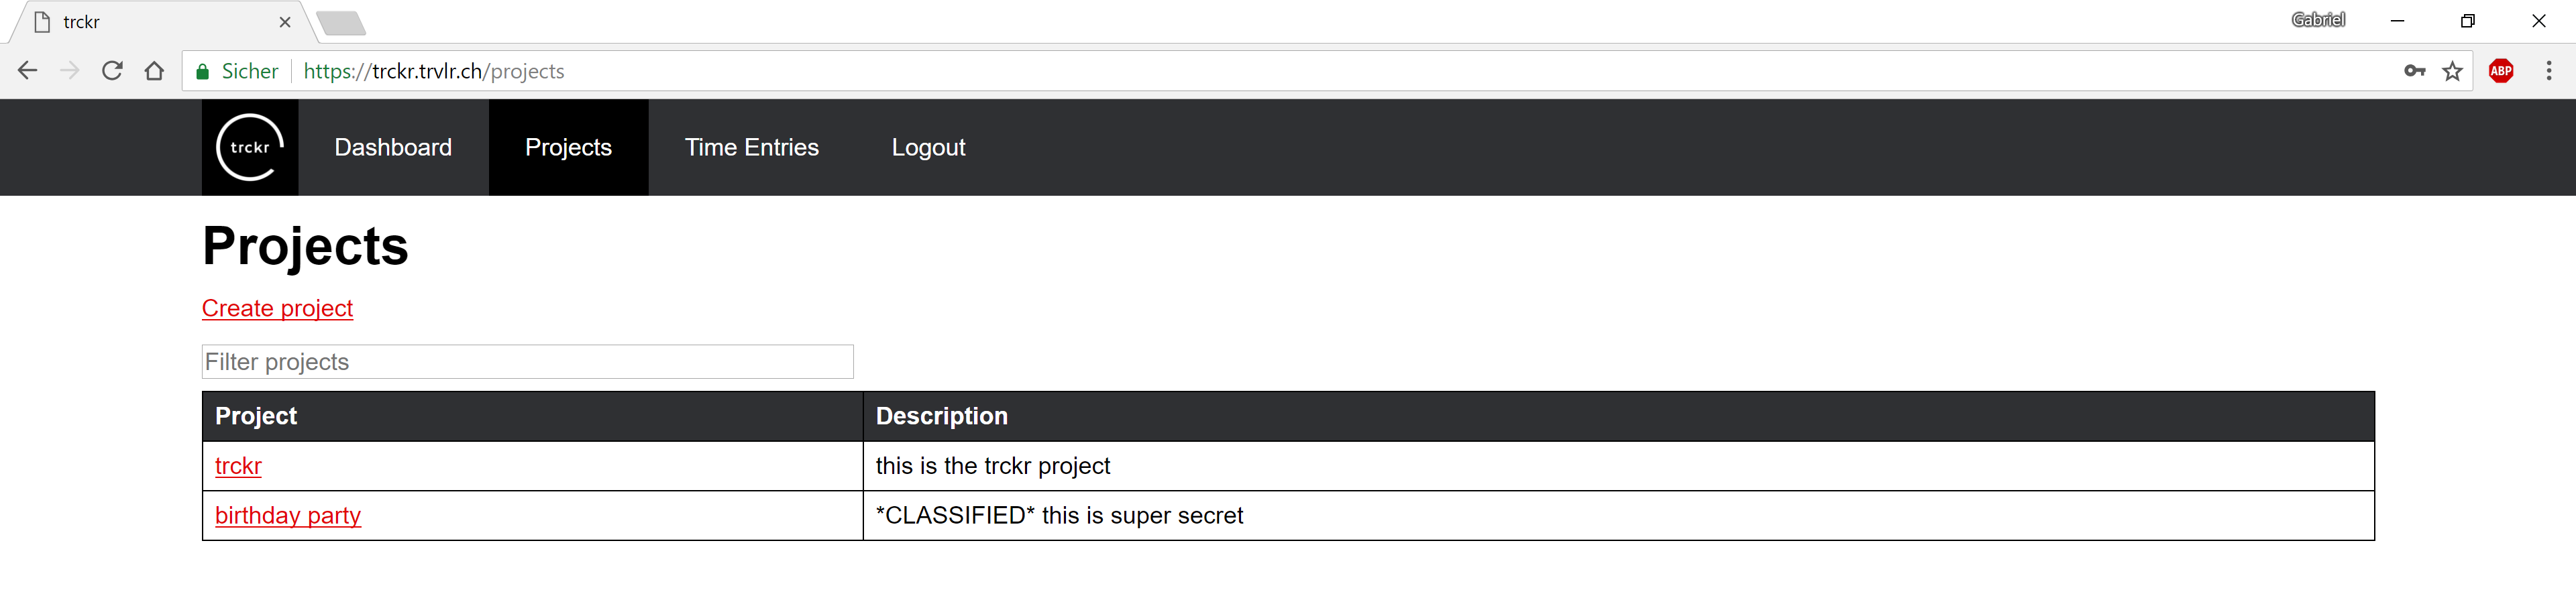
\includegraphics[width=\textwidth]{trckr-projects-table}
    \caption{The dialog to create a new project}
    \label{fig:trckr-create-project}
\end{figure}

Each project can be viewed in more detail by clicking the project name in the
table shown in figure \ref{fig:trckr-project-page}. The project page contains
the name, the description and a table of all the tasks in the selected project.

\begin{figure}[h]
    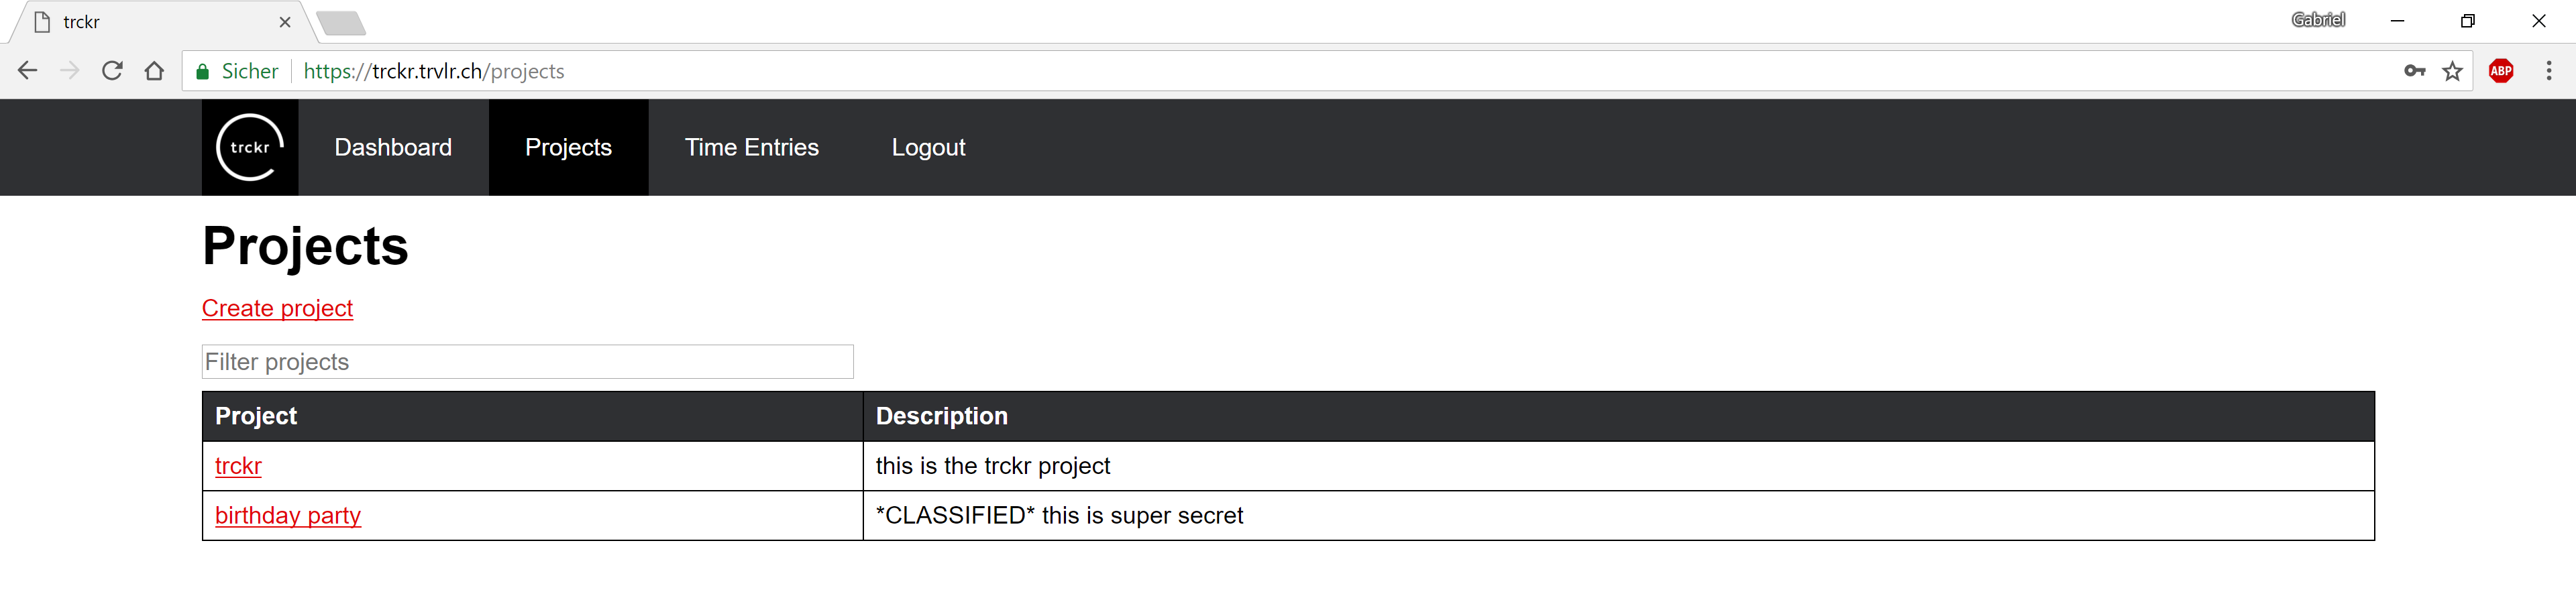
\includegraphics[width=\textwidth]{trckr-projects-table}
    \caption{The projects page with the table containing the projects}
    \label{fig:trckr-projects-table}
\end{figure}

\begin{figure}[h]
    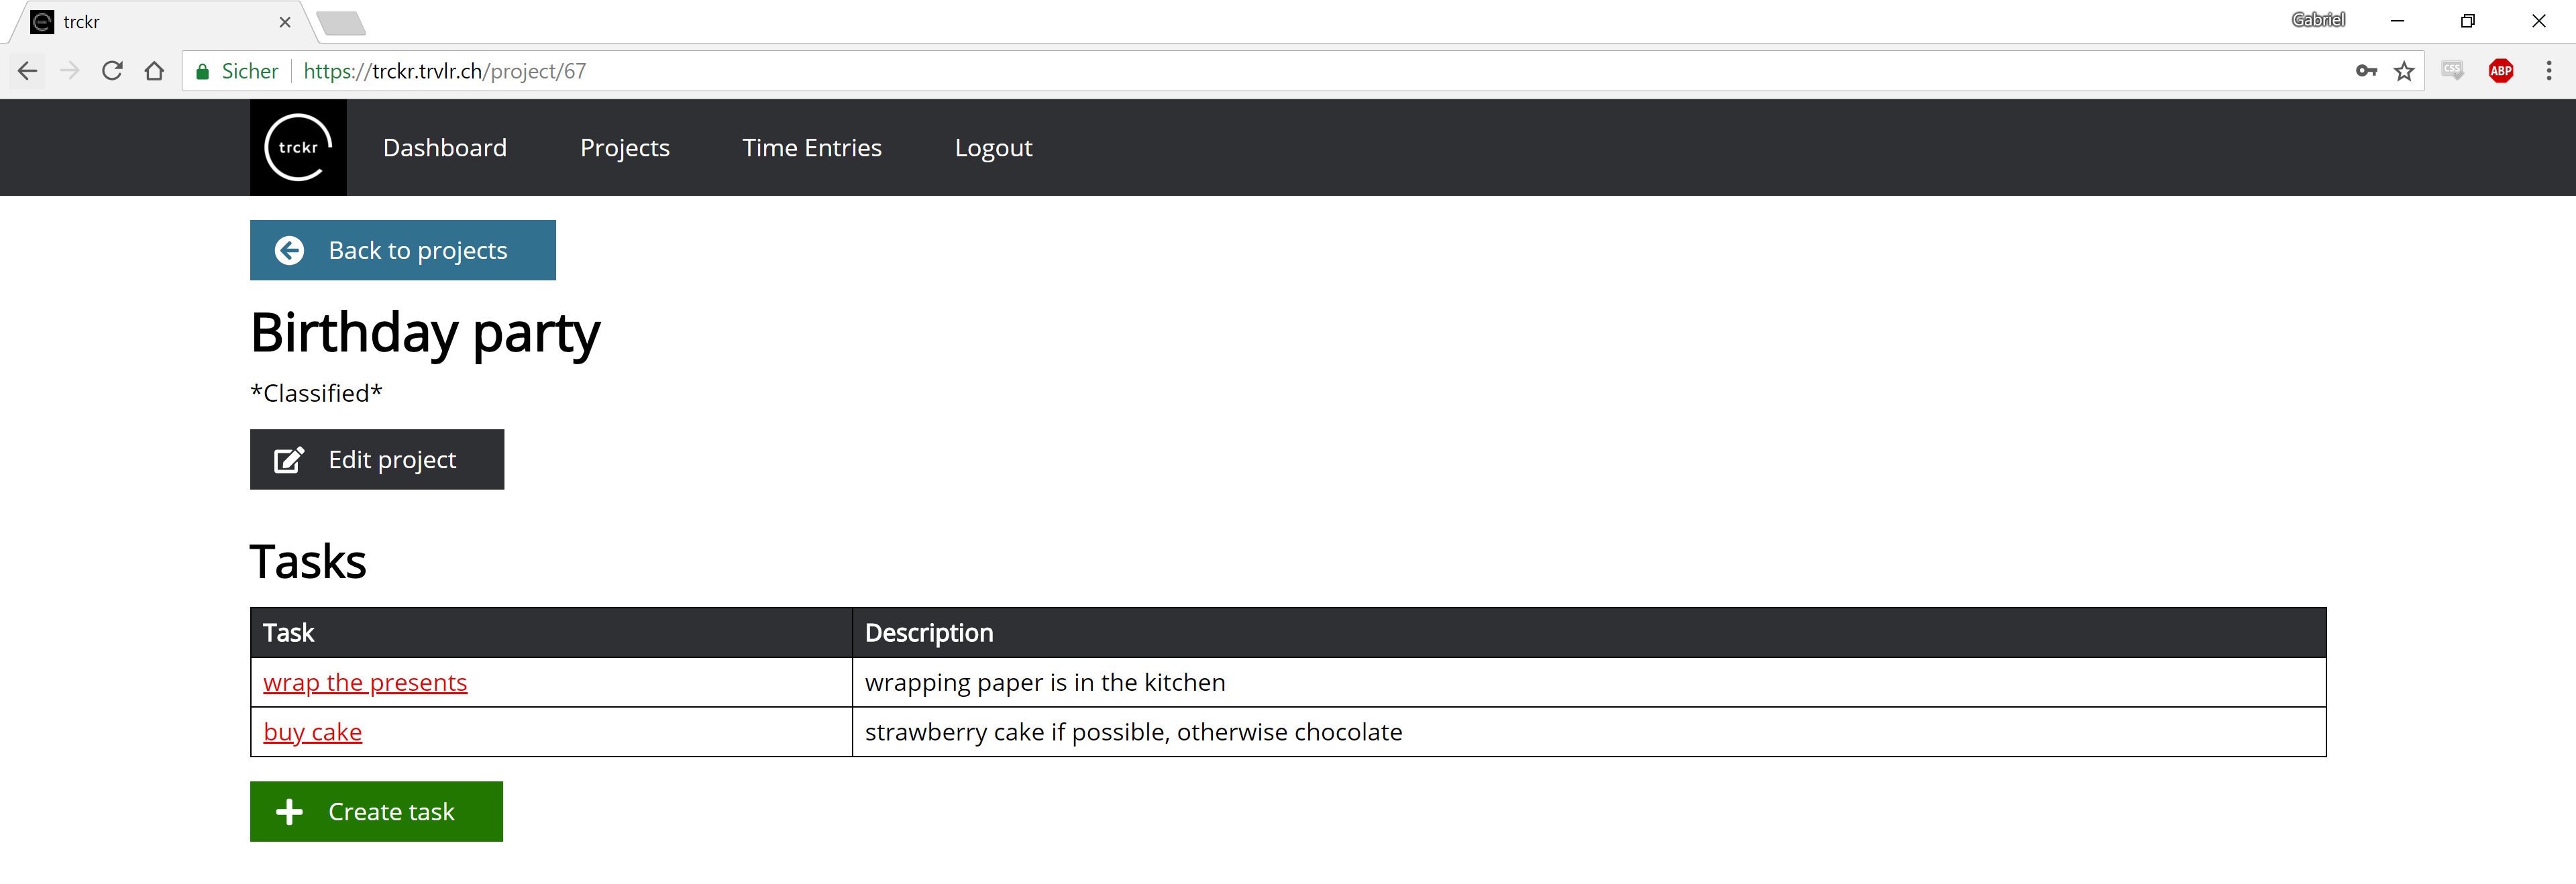
\includegraphics[width=\textwidth]{trckr-project-page}
    \caption{The project page with the table of all tasks}
    \label{fig:trckr-project-page}
\end{figure}

Clicking on a task will display its details like the name and description of
the task.

On the "Time Entries" page, the user can create a time entry for a specific task
of a project with the entry form shown in Figure
\ref{fig:trckr-create-time-entry}. The user selects a project and a corresponding
task for which the time entry should be created.

\begin{figure}[h]
    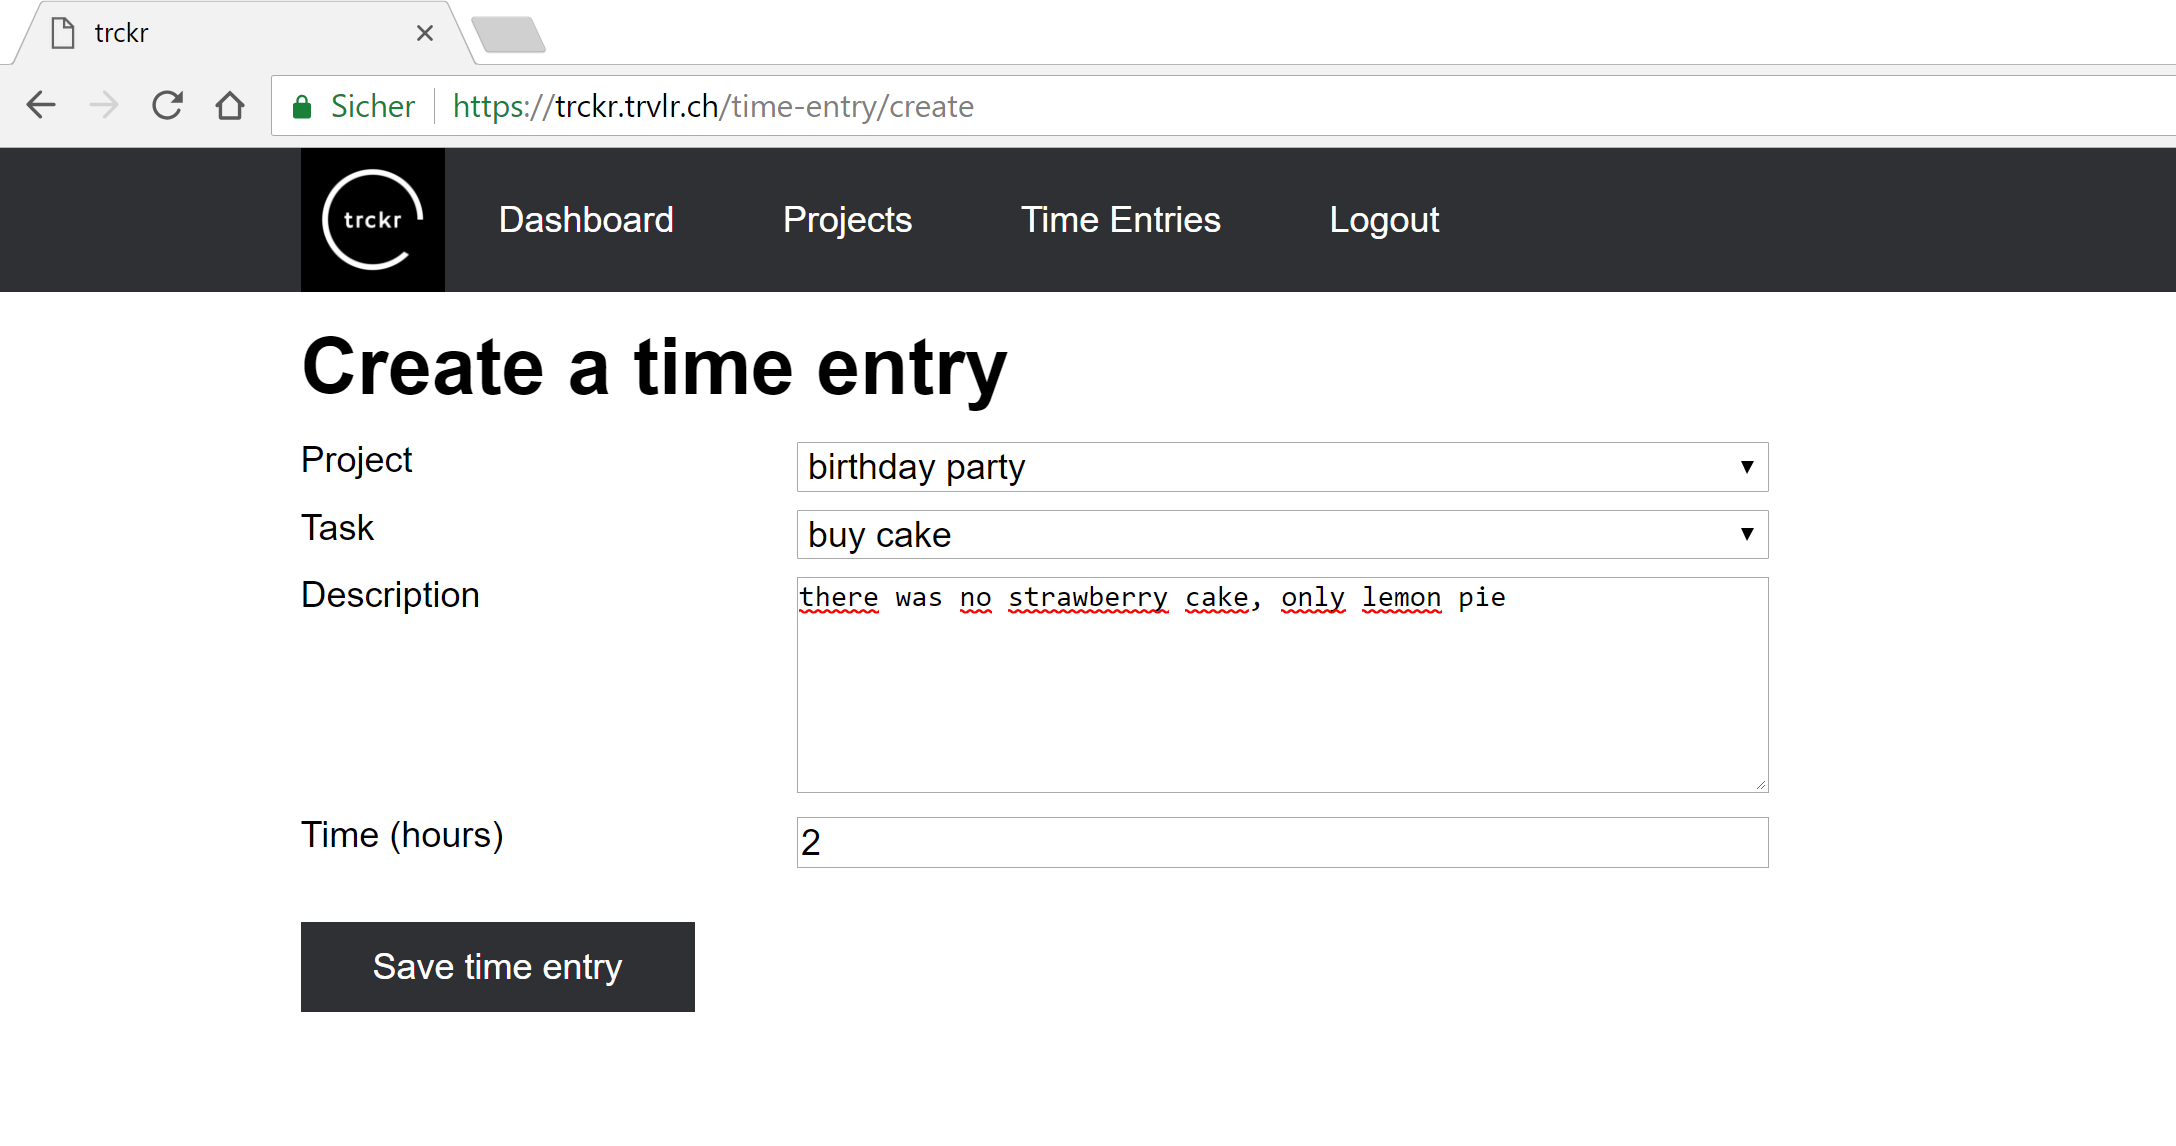
\includegraphics[width=\textwidth]{trckr-create-time-entry}
    \caption{The form to add a time entry to a task.}
    \label{fig:trckr-create-time-entry}
\end{figure}

All time entries will be displayed on the time entry page.

\section{Outlook}
By focusing on doing one thing and doing it right, it was possible to create a
modular platform. This did not just allow a clean development process, but also
enables open-source contributors to easily extend the trckr application. The
main focus now should be to gather real life user experience and feedback to
determine which features should be added next or be improved upon.

Project-focused features can be improved to enable more specific project
methods, maybe even an interface with ticketing or project management tools.
This enables the team leaders to gain more insight on the progress.

A desktop application could be developed to automatically track usage of certain
applications or integrations for development environments to track time worked
on a project. By reducing the manual intervention of the user, the tracking
could become even more accurate. This might even uncover certain inefficiencies,
e.g. by detecting too much time wasted waiting for tests or deployments.

\section{Conclusion}
The aim of the project trckr was to create a tool which helps people and
coorporations to easily track time on their projects. With the help of
sophisticated technologies like Django and Vue.js, the trckr development
team was able to create a modern and responsive web application.

Even though the team had almost no prior experience with the used technlogies,
they proved themselves motivated to invest time to properly learn them. The
agile software development process only helped them to achieve this by providing
clear short-term goals.

The result is a usable web application that can still be improved upon, maybe
even with the help of open-source software developers.

% Appendices
\clearpage
\printbibliography

\end{document}
